\chapter{Decision trees}
\label{chap:decision_trees}

Decision trees~\cite{breiman1984classification,Louppe:14077502} are part of the 
set of \acl{MVA} tools that also includes \acl{kNN} and \aclp{ANN}.
In \acl{HEP}, such tools are commonly used for the task of 
\emph{classification}, where one wishes to discriminate between several species 
that are mixed together, usually in unknown proportions, in the data.
Most generally, the algorithms try to estimate some function whose parameters 
are a set of variables $\vec{x}$, or \emph{features}, and when used for binary 
classification the function is the decision boundary, either side of which is a 
pure sample of each of the two species.
In practice, the generating \acp{PDF} for the species overlap to some degree, 
or the algorithm cannot distinguish them with certainty across the entire 
feature space.
For a given set of values of the features, the algorithm then returns a 
probability that the point $\vec{x}$ belongs to a particular species.
Throughout this \lcnamecref{chap:decision_trees}, only the problem of binary 
classification will be considered.

Rectangular cuts are a crude attempt at estimating the multidimensional 
decision boundary that separates signal from background, with the decision 
being either zero if at least one cut is not passed, or one if all cuts are 
passed.
A decision tree refines this approach by defining cuts which are conditional on 
the outcome of those preceding it.
This begins with a single \emph{node}, the \emph{root}, which defines a cut on 
a single feature $x$, say $x > y$ for some value $y$, by which the input sample 
is split in two.
The sample passing the cut is passed to a node in the next \emph{layer}, whilst 
the failing sample is passed to another node in that layer.
Each of these nodes defines some other cut, possibly on a different feature, 
and the samples are further split and passed to nodes in the next layer.
Each of the $N$ layers can have up to $2^{n - 1}$ nodes, where $n$ is the 
\emph{depth} or layer number.
Eventually the sub-samples can proceed no further and reside in a \emph{leaf}, 
or terminal, node at which point a per-species probability is assigned to them.
An example decision tree is illustrated in 
\cref{fig:decision_trees:decision_tree}.

\begin{figure}
  \centering
  % Adapted from http://www.texample.net/tikz/examples/decision-tree/
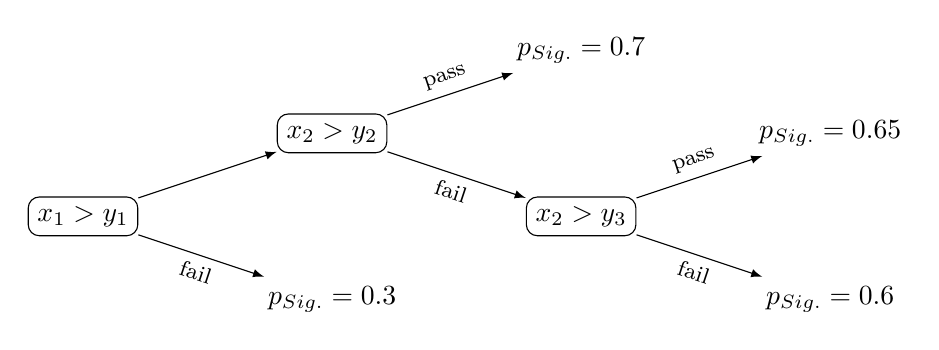
\begin{tikzpicture}
  [
    grow                    = right,
    sibling distance        = 6em,
    level distance          = 9em,
    edge from parent/.style = {draw, -latex,font=\footnotesize},
    sloped,
    treenode/.style = {shape=rectangle, rounded corners,
      draw, align=center},
    root/.style     = {treenode},
    env/.style      = {treenode},
    leaf/.style      = {treenode, draw=white}
  ]
  \node [root] {$x_{1} > y_{1}$}
    child { node [leaf] {$p_{\text{Sig.}} = 0.3$}
      edge from parent node [below] {fail} }
    child { node [env] {$x_{2} > y_{2}$}
      child { node [env] {$x_{2} > y_{3}$}
        child { node [leaf] {$p_{\text{Sig.}} = 0.6$}
          edge from parent node [below] {fail} }
        child { node [leaf] {$p_{\text{Sig.}} = 0.65$}
          edge from parent node [above] {pass} }
        edge from parent node [below] {fail} }
      child { node [leaf] {$p_{\text{Sig.}} = 0.7$}
        edge from parent node [above, align=center]
        {pass} }
    };
\end{tikzpicture}

  \caption{%
    A decision tree, computing signal probabilities $p_{\text{Sig.}}$ in the 
    leaf nodes using a set of features $x_{i}$ and cut values on those features 
    $y_{i}$.
  }
  \label{fig:decision_trees:decision_tree}
\end{figure}

The construction, or growth, of a single decision tree is the process to 
determine which features and cut values are used in what nodes, and what the 
assigned probabilities should be in the terminal nodes.
There are many parameters available for tuning during construction, including: 
the maximum depth; the figure of merit the cut at each node should optimise; 
and the stopping criteria that determines whether additional nodes can be 
created.
Both tuning of these \emph{hyper-parameters} and of the features and cuts to 
use is a complex optimisation problem~\cite{Louppe:14077502}, the details of 
which are not necessary for understanding the classification problem at hand.
The important feature of the construction is that it is performed using an 
ensemble of individual \emph{events}, feature vectors $\vec{x}$, called the 
\emph{training} sample, in which the true species of each event is known.
This is typically a combination of some simulated \ac{MC} sample, known to be 
signal through truth-matching, and some sample from a control region in the 
data which is known to contain no signal, such as mass sidebands.
The decision tree then tries to fit the set of cuts and values such that the 
samples can be classified as cleanly as possible, given the hyper-parameters.
The probability of the terminal nodes can then be taken as, for example, the 
ratio of the two species that remain after the training sample has been passed 
through the final tree.

The discriminating power of a decision tree is driven by two factors: how 
discriminatory the set of features is between the two species; and what are the 
values of the hyper-parameters.
The exact choice of these is dependent on the nature of the classification 
problem, however the hyper-parameters should be chosen such that the decision 
tree is not \emph{over-fitted} to the training data.
This occurs when the tree is too sensitive to the statistical fluctuations in 
the features in the training sample.
It is possible that a tree with infinitely many layers would be able to 
perfectly classify the training sample, for example, but a new signal sample 
not present in the training may be classified as background, as the values of 
the features do not exactly match those in the training sample.
In general, over-fitting results in the performance of the tree being worse on 
an independent \emph{testing} sample, within which the true species are also 
known, than on the training sample.
When tuning the set of hyper-parameters, the performance of the tree should 
then be evaluated on the testing sample.
This is comparable with the normal fitting of functions to data with maximum 
likelihood or \chisq\ methods, in that more complex models can describe the 
data well, to an arbitrary degree for higher complexities, but the models begin 
to offer less general insight, instead being tailored to a specific dataset 
that happens to have been observed.
Measures of performance include the \emph{accuracy}, the number of correctly 
classified events relative to the total number, and the \emph{error rate}, the 
number of wrong predictions relative to the total number.
In the worst case, a classifier does no better at guessing event species than 
uniform random guessing.

The benefit of using decision trees over some other \ac{MVA} algorithms is that 
they can be intuitively interpreted: the tree can be visualised as such, and 
the decisions can be reasoned with by seeing how different features influence 
the lower depths of the tree.
However, a tree that fits the training sample well is in general very deep, as 
only one feature enters the decision in each node.
Deep trees are particularly susceptible to over-fitting, and so \emph{ensemble} 
methods are often used.

\subsection{Ensembles of trees and boosting}
\label{chap:decision_trees:boosting}

The error rate of a decision tree, the fraction of incorrectly classified 
events, is due to two properties of the classifier: the bias, the consistent 
deviation away from the true values, and the variance, the spread around the 
mean value~\cite{Breiman96biasvariance}.
A complex model, prone to over-fitting, may have a low bias but a high 
variance, whereas a simple model may have a high bias but a low variance.

To reduce the variance of a tree-based classifier, ensembles of complex trees 
can be created, where each tree is grown using a subset of the training 
data~\cite{Breiman1996}.
The classification for an event is then determined using the set of 
classifications produced by the ensemble, such as by taking the mean of that 
set.
This does not increase the bias of the model if the predictions of the 
individual trees are uncorrelated.
To guard against this possibility, the technique of \emph{random 
  forests}~\cite{Breiman2001,Louppe:14077502} can be used, in which each node 
splitting can only use information from a random subset of the features, in 
addition to the random sub-sampling of the training data used to grow each tree 
in the ensemble.

The bias can be decreased by employing \emph{boosting}, for which 
\adaboost~\cite{Freund1997119} is a commonly used algorithm.
Rather than training an ensemble of complex models in parallel, \adaboost\ 
trains a \emph{sequence} of \emph{weak learners} (decisions trees here), whose 
predictions are only slightly better than random guessing, and returns a 
weighted sum of their predictions as the final classification.
This begins by growing a single, shallow tree where the $i$th vector in the 
training sample is weighted with a weight $w_{i} = 1/N$.
The training sample is fed through the tree, and events which were classified 
incorrectly are assigned a larger weight, and those which were classified 
correctly are assigned a smaller weight.
A new tree is grown using the new weights, and the procedure is iterated.
With each iteration, events that are consistently incorrectly classified are 
given a greater importance in the training.

The generalisation of the \adaboost\ algorithm is \emph{gradient 
  boosting}~\cite{friedman2001}.
With \adaboost, additional weak learners compensate for previous incorrect 
classifications by being trained with specially weighted data.
In gradient boosting, additional weak learners try to correct the 
classification of the previous learners by fitting a regression model 
$f(\vec{x})$ to the residuals ${(\hat{y}_{i} - f(\vec{x}_{i}))}^2$ of the 
predicted classification $f(\vec{x}_{i}) = y_{i}$ and the true classification 
$\hat{y}_{i}$.
In this way, gradient boosting tries to minimise the \emph{loss function} that 
characterises how poorly the classifier is performing, and can be generalised 
by considering an arbitrary loss function $L(\hat{y}, f(x))$, which can be the 
residual.
